\section{Introduction}

La plupart des langages de programmation offrent les mêmes types pour stocker des nombres. Il s'agit notamment des nombre entiers et des nombres réels. Ces nombres réels sont toujours en virgule flottante.

Ces types ont tout de même des limitations. Les nombres sont limités en taille et au domaine du réel. Quant à eux, les nombres à virgule flottante sont inexacts. Par conséquent, lorsque les erreurs s'accumulent, le résultat d'un calcul peut être complètement faux sans qu'on le sache.

Pourtant, d'autres alternatives existent. Les nombres complexes sont couramment utilisés en mathématique et en physique. Quant à eux, les nombres réels peuvent aussi être représentés avec des Unum.


\section{Contexte}

En Java, aucun type ni aucune classe dans le JDK permet de gérer des nombres complexes ou des Unum.

Si on veut ajouter ces types, on pense naturellement à créer ces objets. Cependant il est aussi possible de \todo{...}

COJAC \cite{COJAC} est une librairie Java permettant de modifier les capacités arithmétiques d'un programme Java sans en modifier le code.

\section{Objectifs}

Le but de ce projet est d'ajouter deux nouvelles fonctionnalités à COJAC \cite{COJAC}.

\subsection{Intégration des nombres complexes}

Une option de COJAC permettra de changer le comportement des calculs dans l'application de l'utilisateur. Les calculs se feront ainsi avec des nombres complexes.

\subsection{Intégration des Unum}

Une option de COJAC permettra de changer le format de stockage des nombres réels. Les Unum seront utilisés à la place de la virgule flottante.

\subsection{Démonstration des deux fonctionnalités}

Des démonstrations seront réalisées pour les montrer l'utiliser des deux fonctionnalités.

\section{Objectifs secondaires}


\subsection{Mise à jour des librairies}

COJAC \cite{COJAC} utilise plusieurs vielles librairies. Ce serait bien de les mettre à jour si possible.

\subsection{Tests de performance}

Des tests de performance peuvent aussi être effectués pour tester l'efficacité de l'implémentation.

\section{Tâches}

Cette section détaille les tâches qui devront être effectuées pour réaliser chacun des objectifs définis précédemment.

\subsection{Intégration des nombres complexes}

Les tâches suivantes seront effectuées pour réaliser cet objectif:
\begin{itemize}
    \item Analyse des implémentations existantes.
    \item Analyse de COJAC et de comment intégrer un nouveau type.
    \item Analyse des nombres complexes.
    \item Concevoir l'algorithme.
    \item Implémenter l'algorithme.
    \item Tester l'algorithme.
\end{itemize}

\subsection{Intégration des Unum}

Les tâches suivantes seront effectuées pour réaliser cet objectif:
\begin{itemize}
    \item Analyse des implémentations existantes.
    \item Analyse de COJAC et de comment intégrer un nouveau type.
    \item Analyse des Unum.
    \item Concevoir l'algorithme.
    \item Implémenter l'algorithme.
    \item Tester l'algorithme.
\end{itemize}

\subsection{Démonstration}

Les tâches suivantes seront effectuées pour réaliser cet objectif:
\begin{itemize}
    \item Imaginer une situation pour les démonstrations.
    \item Réaliser les démonstrations.
\end{itemize}

\subsection{Mise à jour des librairies}

Les tâches suivantes seront effectuées pour réaliser cet objectif:
\begin{itemize}
    \item Chercher les mises à jour de chaque librairie.
    \item Regarder les changements avec la nouvelle version.
    \item Modifier la version et adapter le code.
    \item Tester les modifications.
\end{itemize}

\subsection{Tests de performance}

Les tâches suivantes seront effectuées pour réaliser cet objectif:
\begin{itemize}
    \item Analyser les tests de performance actuels.
    \item Réaliser les tests de performance.
\end{itemize}

\begin{landscape}
\section{Planification}
La figure \ref{fig:gantt} montre le diagramme de Gantt avec la liste des jalons et des tâches.
\begin{figure}[h!]
   \centering
    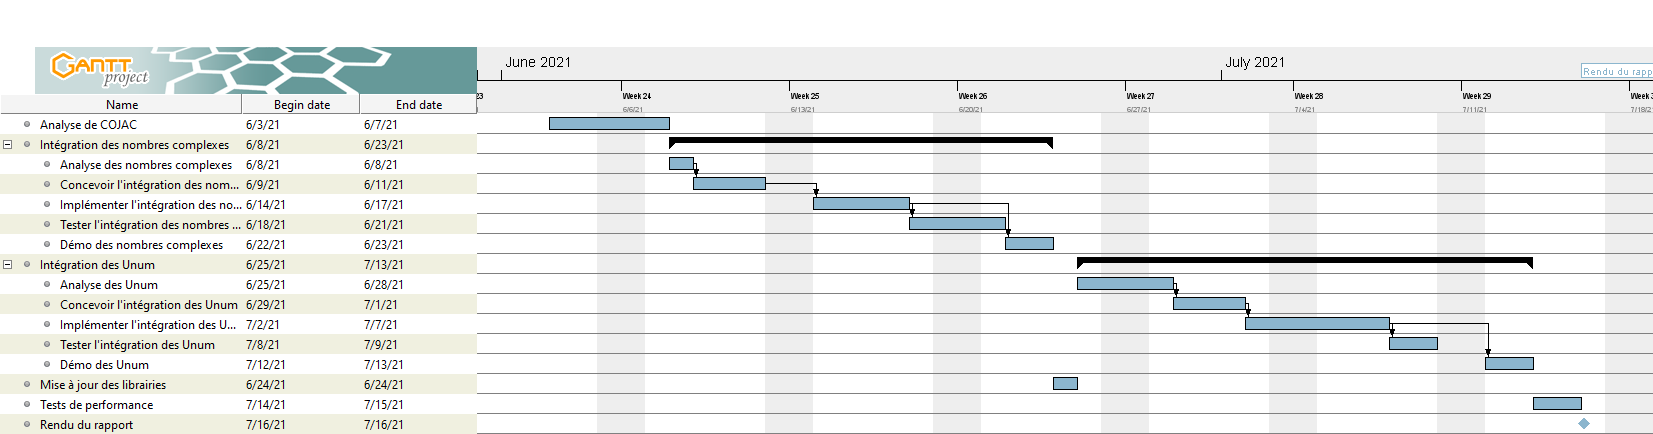
\includegraphics[width=0.98\linewidth]{planning.png}
    \caption{Diagramme de Gantt}
    \label{fig:gantt}
\end{figure}

\end{landscape} 